
\(f(x) = 3x\e^{-0{,}4x}\).

\subsection*{1.}

Comme quel que soit le réel \(x\), \(\e^{-0{,}4x} > 0\), le signe de \(f'(x)\) est celui de \(-1{,}2x + 3\).
\begin{align*}
&-1{,}2x + 3 > 0 \\
\iff &3 > 1{,}2x \\
\iff &x < 2{,}5.
\end{align*}
Sur \([0 \,;\, 2{,}5[\), \( f'(x) > 0 \), sur \(]2{,}5 \,;\, +\inf[\), \( f'(x) < 0 \) et \( f'(2{,}5) = 0 \).

\subsection*{2.}

La fonction est donc croissante sur l'intervalle \(]0 \,;\, 2{,}5[\) et décroissante sur \(]2{,}5 \,;\, +\infty[\).

\[
f(2{,}5) = 3 \times 2{,}5 \times \e^{-0{,}4 \times 2{,}5} = 7{,}5 \e^{-1} \approx 6{,}79.
\]

\begin{center}
\begin{tikzpicture}
\tkzTabInit[lgt=3.5, espcl=4]{$x$ / 1, {Signe de $f'(x)$} / 1, {$f(x)$} / 2}{${0}$, ${2{,}5}$, ${+\infty}$}
\tkzTabLine{,+,0,-,}
\tkzTabVar{-/{$$},+/{$7{,}5\e^{-1}\approx 6{,}79$},-/{$$}}{/}
\end{tikzpicture}
\end{center}

\subsection*{3.}

\paragraph{a.} On a au temps 0, jour de l'ingestion dans l'organisme du sportif, la quantité de produit dopant égale à : \(3 \times 0\e^0 = 0\).

\paragraph{b.} De la question 2. on déduit que la quantité maximale du produit dans l'organisme est détectable au bout de 2 h 30 min.

\paragraph{c.} On a : \(C(6) = 3 \times 6\e^{-0{,}4 \times 6} = 18 \e^{-2{,}4} \approx 1{,}633\).

Comme \(1{,}633 > 1{,}4\), le sportif sera détecté positif.

